\chapter{Smaller organisms are less strongly structured by environmental variation}
\label{chap:organism-size}

\section{Introduction}\label{introduction}

One of the most profound differences between organisms is their body
size. Small and large organisms can differ in population size, growth
rates, morphological complexity, genome size, and modes of dispersal.
This scaling of biological processes with organism size has often been
used to explain differences in the spatial distribution of small and
large organisms. Microscopic organisms such as bacteria and plankton are
often globally distributed, while larger organisms have more
geographically restricted distributions \citep{Fenchel2004}. Even within
landscapes, there is some evidence that the occurrence of such
microscopic organisms responds less to environmental gradients than does
the occurrence of larger organisms \citep{Farjalla2012, Fierer2011}.
However, while such differences in distribution suggest that the suite
of processes underlying community assembly differ between small and
large organisms, it is difficult to determine which process is driving
this difference. There are at least two possible mechanisms that may
make communities of smaller organisms more widely distributed. First,
smaller organisms could have larger environmental tolerances, allowing
them to occupy broader fundamental niches. Second, smaller organisms
could have greater dispersal abilities, allowing them to reach more
habitats.

Smaller organisms may have broader environmental tolerances for several
reasons. First, their small body size allows habitat heterogeneity to
affect them at very small scales: smaller organisms are able to find
tolerable microhabitats, while organisms that experience the environment
at a coarser grain may not detect a similar variation in the
environment. This biological difference between small and large
organisms can be compounded by the macroscopic grain at which organisms
are typically observed by researchers, which averages over any
microscopic-scale variation in distribution. Secondly, single-celled
organisms may be able to use multiple carbon sources
\citep{Langenheder2007} allowing them to survive in a greater range of
habitats. Very small organisms are also more likely to possess resting
stages when a habitat is unfavorable (e.g.~cysts for protists, tun state
for tardigrades) or to propagate by means of a resistant life history
stage such as spores. At the population level, small organisms may
persist in a habitat if they are able to adapt to local conditions by
virtue of their short generation times and high population sizes. In the
case of bacteria, genetic adaptation can also involve the uptake and use
of environmental DNA.

Alternatively, small organisms may be widely distributed because they
are able to get to more places faster. There is substantial evidence
that microscopic organisms such as bacteria, viruses, protists and
plankton may be able to disperse further than larger organisms; amongst
these microscopic organisms, the smallest disperse the furthest. The
classic ``everything is everywhere and the environment selects''
hypothesis of Baas Becking \citeyearpar{BaasBecking1934} suggests that
smaller organisms are not limited by dispersal barriers or distance but
instead are found globally, emerging from resistant stages in favorable
environments \citep{Huszar2015}. Many bacteria and zooplankton have
passive dispersal, traveling long distances by wind or water currents,
or by phoresy. In contrast, larger animals (but not larger plants)
usually have active dispersal; for example, adult insects actively
choose sites to oviposit. At the scale of landscapes, active dispersal
could result in a close association between distribution and
environmental variables, assuming that active dispersal behaviour is
adapted to maximize fitness. However, at continental and global scales,
the limited distances covered by active dispersers might prevent larger
animals from reaching suitable places. This would weaken the association
between environment and distribution for larger animals.

It has been difficult to determine whether differences in distribution
between small and large organisms is caused by differences in the
strength of environmental filtering or dispersal limitation. There are
three reasons for this. First, the distribution of micro-and macroscopic
organisms has rarely been compared within the same system. This creates
a problem of scale, with studies of many macroscopic organisms occurring
on much smaller spatial scales than those of microscopic organisms.
Second, when we rely on observational data alone, we have a limited
ability to infer environmental filtering. This is because environment,
space and dispersal are often correlated. Previous researchers have used
variance partitioning to separate the effects of environment from space,
but this approach has limitations \citep{Gilbert2010}. For example,
Smith and Lundholm \citeyearpar{Smith2010} found that
spatially-correlated dispersal contributed to both spatial and
environmental partitions of variance in community composition. Third,
dispersal limitation and environmental filtering can mask each other. A
species can only be filtered by a site's environment when it can reach
the site, so a community experiencing equally strong dispersal and
environmental limitation can may show mainly the former in variance
partitioning \citep{Smith2010, DeBie2012a}. A special case of this
problem occurs when an actively-dispersing species is not found in a
site. It is impossible to determine if this is because the environment
makes dispersal unlikely or establishment unlikely. For example, an
insect larva may be missing from a location because its parent was
deterred from ovipositing in the environment or because the larvae could
not withstand the environment. An experiment that removes dispersal
limitation for all organisms is therefore a stronger test of the
relative effects of environment on species composition. We are aware of
no study that experimentally removes dispersal limitation for both
micro- and macroscopic organisms in the same system, simultaneously, to
reveal environmental filtering. We conducted such an experiment, using
bromeliad phytotelmata as a model community.

Here we provide a robust test of the strength of environmental filtering
for these three organism types by experimentally dispersing all species
to all habitats, and examining whether the original habitat-based
patterns in composition re-emerged. We predicted:

\begin{enumerate}
\def\labelenumi{\arabic{enumi}.}
% \tightlist
\item
  If environmental filtering, but not dispersal limitation, increases
  with organism size, we would predict that habitat would affect the
  composition of communities of large-bodied organisms more than those
  of small-bodied organisms(Figure \ref{fig:illustration}a). 
\item
  If instead only dispersal limitation increased with organism size, we
  would expect that any apparent effect of habitat on community
  composition was an artifact of spatial autocorrelation and would be
  erased by our removal of dispersal limitation (Figure \ref{fig:illustration}b).
\item
  If both environmental filtering and dispersal limitation increased
  with organism size, we would predict an intermediate scenario (Figure
  \ref{fig:illustration}c).
\end{enumerate}

\subsubsection{Study system}\label{study-system}

Bromeliads are common in the Neotropics and contain many species of
macroinvertebrates, especially insects \citep{Frank2009}, zooplankton
\citep{Petermann2015}, and bacteria \citep{Haubrich2009a}. Importantly,
different species of bromeliad grow in different habitats, and this
habitat variation is correlated with differences among their communities
\citep{Marino2012}. Previous observations in this system show that this
environmental variation is closely associated with variation in
macroinvertebrate composition, weakly associated with variation in
zooplankton communities and almost uncorrelated with variation in
bacterial communities \citep{Farjalla2012}.

\begin{figure}[htbp]
\centering
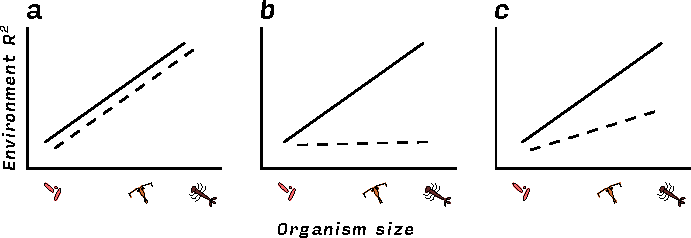
\includegraphics[width=5.5in]{figures/hypotheses_illustration.pdf}
\caption[Illustration of the possible patterns resulting from our
experiment.]{Illustration of the possible patterns resulting from our
experiment. Previous observations have already shown that community
composition of larger animals is more strongly related to environmental
differences than is composition of smaller organisms (solid line, all
figures). In our experiment we remove differences among community
composition, and observe the subsequent return of these differences as
caused by environment (dashed lines). There are three possible outcomes.
If differences in composition are caused by an increase in sensitivity
to the environment (with increasing organism size), then we should see a
match between the amount of environmental signal before and after the
experiment (1a). If differences in composition are caused by biased
dispersal, we should see no difference between organism types after the
experimental homogenization (1b). Finally, an intermediate scenario (1c)
results when both environment and biased dispersal contributed to the
original pattern.}
\label{fig:illustration}
\end{figure}

\section{Methods}\label{methods}

\subsubsection{Experimental design}\label{experimental-design}

We performed this experiment in the same location and along the same
gradient of environmental variation (bromeliad species in different
habitats) as Farjalla et al. \citeyearpar{Farjalla2012}. Both their
study and ours took place in the Parque Nacional de Jurubatiba,
Northeast Rio de Janeiro state, Brazil (\(22^{\circ}\) S \(41^{\circ}\)
W). The environmental gradient in this ecosystem is twofold -- three
different species of bromeliad, which differ also in their preferred
level of exposure to sunlight: \emph{Aechmea nudicaulis} (full sun
habitats), \emph{Vriesea neoglutinosa} (partial shade), and
\emph{Neoregelia cruenta} (full shade). \emph{Neoregelia} has a uniquely
large habitat range at this site, occurring in both full shade and full
sun; only shade plants were used in this study.

For each of five temporal blocks, we collected and sampled the
macroinvertebrates, zooplankton and bacteria of two bromeliads of each
of the three species. We then homogenized the communities of all six
bromeliads as described shortly (Figure \ref{fig:schematic}). Our goal was to create
identical starting community composition for all bromeliads within a
block. Variation between blocks in starting community composition is
thus included in the random effect of blocks. We created five blocks in
this experiment between 27 March 2013 and 03 April 2013.

\begin{figure}[htbp]
\centering
\includegraphics[width=5.5in]{figures/design_illustration.pdf}
\caption[Schematic of experimental design.]{Schematic of our experimental design. We first sampled six bromeliads (two plants of each of three species). We formed (solid
arrows) homogeneous initial communities (MIX) by counting equal numbers
of animal taxa (macroinvertebrates) or by mixing water samples of equal
volume from all plants (zooplankton and bacteria). We then returned
(dashed arrows) initial communities to the six bromeliads in their
associated habitats.}
\label{fig:schematic}
\end{figure}

Our experimental setup consisted of three steps (Figure \ref{fig:schematic}): collection
of original communities from bromeliads, homogenization of communities,
and assembly of this homogenized community in each of the original (now
empty) bromeliads. \textbf{Original communities}: We sampled the
zooplankton and bacteria communities by collecting water samples from
each bromeliad: 100ml for zooplankton, 50ml for bacteria. Zooplankton
were collected by filtering on 50 μm Nytex mesh and fixed in 5\%
buffered formalin. This fixed solution was then diluted to 20 ml, and a
1 ml subsample taken for analysis. Zooplankton were identified to the
lowest taxonomic unit possible (species in most cases, except for
bdelloid rotifers and harpaticoid copepods, identified to class and
order, respectively). Bacteria were collected by taking 100ml of
filtrate from the zooplankton sample and filtering it a second time on a
Whatman filter paper. We measured bacterial community composition using
denaturing gradient gel electrophoresis (DGGE, Muyzer et al.
\citeyearpar{Muyzer1993}). This technique measures an approximation of
bacterial diversity in the form of Operational Taxonomic Units (OTUs).
We sampled macroinvertebrates by thoroughly rinsing each bromeliad and
filtering the water through two sieves (1 millimeter and 180 micrometer). These mesh sizes have
been shown to separate macroinvertebrates from both coarse detritus and
fine particulate organic matter, facilitating their collection
\citep{Romero2010}. We identified macroinvertebrates to morphospecies.
\textbf{Homogenized communities}: We created homogenized communities of
zooplankton and microbes by mixing an equal volume of filtered tank
water from each of the six bromeliads in a block (approximately 100ml
plant\textsuperscript{-1}), then adding this mixture to all bromeliads.
To create homogenized communities of macroinvertebrates, we divided
individuals of all species equally among the six bromeliads in each
block. \textbf{Bromeliad preparation}: We emptied bromeliads by washing
them thoroughly, hanging them upside down to dry for at least 24 hours
and then rinsing each plant with 70\% ethanol. We confirmed that this
technique removed all invertebrates and most detritus by dissecting an
empty bromeliad. Any coarse detritus found in the bromeliads was
similarly cleaned, frozen and thawed (to kill any eggs or resting stages
of macroinvertebrates).Bromeliads were placed in a local habitat similar
to their original location: \emph{Neoregelia} in shade, \emph{Aechmea}
in full sun and \emph{Vriesea} in marginal habitat. We then added the
starting communities of macroinvertebrates, zooplankton and bacteria.

Bromeliads are an open system, characterized by continual colonization
and emergence. Both of these processes are problematic for our question.
If we were to allow colonization it could swamp any changes in our
starting community composition. Conversely, if we allowed the experiment
to continue for too long any macroinvertebrates with complex life cycles
would emerge, leaving us with no community to sample \citep{Lecraw2014}.
We took two steps to make sure that our treatment effects were not
affected by colonization or excessive emergence. To prevent colonization
we surrounded bromeliads with mosquito netting (mesh size approx. 1.5
mm). To prevent emergence we ended our experiment after 12 days, based
on the results of a pilot study that confirmed that this was sufficient
time for communities to change, but not so long that bromeliads became
empty of organisms

\subsubsection{Analyses}\label{analyses}

We distinguished between our three predictions (Figure \ref{fig:illustration}) with a
permutational ANOVA (PERMANOVA), which measures the amount of difference
in community composition between treatment groups and compares this to
the expected distribution under a null hypothesis of no treatment
effects. In each PERMANOVA we used block as an error stratum, meaning
that permutations were performed within blocks. We repeated this
analysis for all three organism types, and at both ``initial'' and
``final'' sampling dates (i.e.~at the beginning and end of the
experiment). We interpreted the R\textsuperscript{2} value of this
PERMANOVA as a metric of the strength of habitat filtering (Figure \ref{fig:illustration}).
Our hypothesis predicted that R\textsuperscript{2} values should
increase from smaller to larger organism types. However, because we
sampled each of these groups with different techniques, and collected
different types of data (e.g.~abundance data for macroinvertebrates,
presence/absence for bacterial OTUs) we may observe different
R\textsuperscript{2} values through statistical, not biological,
processes. Therefore we tested a pattern of increasing
R\textsuperscript{2} against the increase that would be expected under
the null hypothesis of no difference in environmental filtering. We
first quantified the upward trend with the slope of a linear regression
of R\textsuperscript{2} as a function of approximate organism size
(bacteria = 0.04mm, zooplankton = 0.5mm, macroinvertebrates = 5mm). To
generate our null distribution, we generated a random permutation of the
environmental variable (i.e.~bromeliad species). We used the same
permutation series for each organism type. We calculated the
standardized effect size of the observed slope with the equation

\[SES = \frac{Slope_{observed} - mean(Slope_{null})}{SD(Slope_{null})}\]

We calculated the null p-value as the proportion of null simulations
equal or greater to the observed slope. All statistical analyses were
conducted in R 3.2.3 \citep{rcore}.

\section{Results}\label{results}

Bromeliad species identity explains more variation in community
composition of macroinvertebrates than any other organism type, less for
zooplankton and less still for bacteria (Figure \ref{fig:r2test}, Table \ref{tab:rsquares}). For all
organism types, bromeliad species explained less of the variation in
composition at the end of the experiment than at the beginning. Note
that, although the sampling design (and therefore degrees of freedom)
are identical for all groups, the critical (alpha = 0.05) F-value for
each organism group differs because PERMANOVA p-values are calculated on
a null distribution generated by permuting samples among groups (species
in our case). Bacterial communities have many species and also high
similarity among communities (bromeliads), creating a null distribution
with low mean and small variance (and hence lower thresholds for
significance). This increases the power to detect habitat effects for
bacteria, explaining why this group has marginally significant effects
of habitat despite habitat explaining a tiny amount of total variation
in composition.

So far, we have assessed the absolute effect of habitat filtering on
each organism group separately, but our goal was also to determine if
the strength of habitat filtering increases between the organism groups.
We therefore compared this pattern of increasing environmental effects
with a null model. First, we calculated the slope of the relationship
between the R\textsuperscript{2} value and approximate organism size. We
then generated null distributions by reshuffling bromeliad species
within blocks, using the same permutation across all organism types. We
found that the observed slope was much higher than the null simulations
for both initial (SES = 6.18, p = 0.002) and final (SES = 4.82, p =
0.002) sampling (499 simulations).


\begin{table}[h]
\centering 
\begin{tabular}[c]{r l l l l} 

\toprule
                   &         & F\textsubscript{2,27} & p & R\textsuperscript{2} \\
\midrule
macroinvertebrates & before  & 7.03 & 0.001 & 0.34 \\
                   & after   & 6.42 & 0.001 & 0.32 \\
zooplankton        & before  & 2.59 & 0.008 & 0.16 \\
                   & after   & 1.75 & 0.158 & 0.11 \\
bacteria           & before  & 0.69 & 0.085 & 0.05 \\
                   & after   & 0.63 & 0.027 & 0.04 \\
\bottomrule
\end{tabular}
\caption[Bromeliad species effects on the composition of three groups of organisms]{Bromeliad species effects on the composition of three types of
organisms, as determined by PERMANOVAs both before and 12 days after
homogenization. Both before and after homogenization,
R\textsuperscript{2} values (our proxy for the strength of habitat
filtering) are higher for macroinvertebrates than for zooplankton than
for bacteria. Following homogenization, macroinvertebrate and bacterial
communities both significantly diverged among bromeliad species.} 
\label{tab:rsquares} 
\end{table} 

\begin{figure}[htbp]
\centering
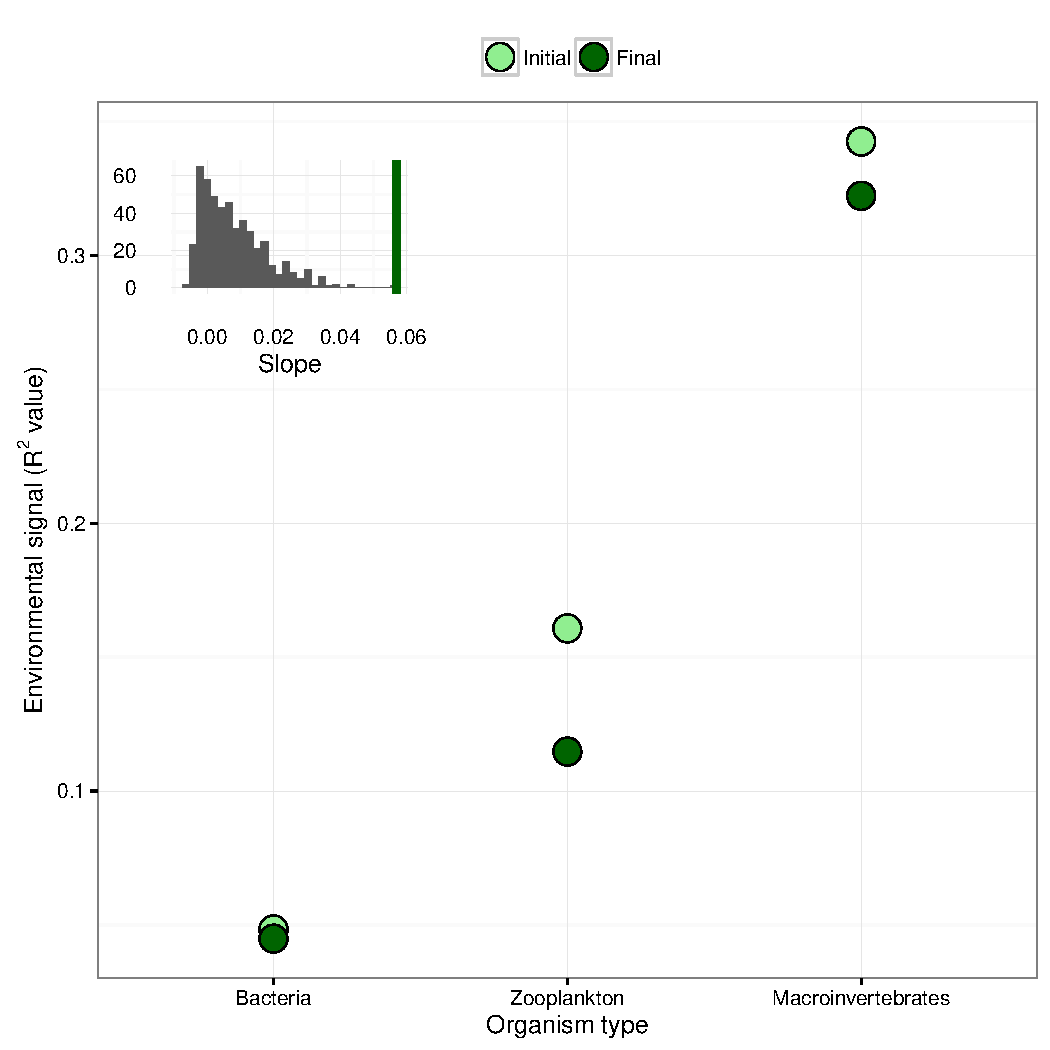
\includegraphics[width=5.5in]{figures/r2_plot.pdf}
\caption[Bromeliad species explains more variation in community composition in larger organisms.]{The amount of variation (R\textsuperscript{2} from PERMANOVA)
in community composition explained by bromeliad species (i.e.~the
strength of the environmental signal) decreases from larger to smaller
organisms. The environmental signal in initial, undisturbed communities
was removed by homogenization, but after 12 days of recovery, was again
of similar strength in final macroinvertebrate and bacterial
communities. Inset shows the results of a null simulation to test the
significance of this increase in R\textsuperscript{2} value: histogram
is the distribution of slopes (R\textsuperscript{2} as a function of
approximate organism size) and the dark green line indicates the
observed value of the slope for the \emph{Final} sampling.}
\label{fig:r2test}
\end{figure}

\section{Discussion}\label{discussion}

\subsubsection{Main findings}\label{main-findings}

Our study compared the response of macroinvertebrates, zooplankton and
bacterial communities to an identical environmental gradient. Our
initial sampling prior to the experimental manipulation found that the
correlation between environment and community composition is weakest for
bacteria, intermediate for zooplankton, and strongest for
macroinvertebrates (Figure \ref{fig:r2test}). This observational pattern mirrors that
previously reported by Farjalla et al. \citeyearpar{Farjalla2012},
confirming that the observational pattern is robust to differences in
field site and year. However, this observed pattern may have been caused
by differences among the three organism types in the strength of
environmental filtering or environmentally-correlated dispersal, or both
(Figure \ref{fig:illustration}). We therefore removed dispersal limitation among communities
by homogenizing our starting communities, and then returned communities
to the same environmental gradient to test whether pure environmental
filtering was sufficient to restore the initial pattern in
distributions. Our results are most consistent with environmental
filtering increasing with organism size (Fig 1a). Specifically, we found
that the environment created minimal differences in bacteria, weak
differences in zooplankton, and large differences in macroinvertebrates
(Figure \ref{fig:r2test}).

Our experimental manipulation suggests that environmental filtering is
stronger for larger than smaller organisms, and that this explains the
differences observed in the field between organismal groups. An increase
in environmental filtering with body size is most simply explained as a
contraction in the breadth of the fundamental niche as organism body
size increases. Farjalla et al. \citeyearpar{Farjalla2012} termed this
hypothesis the ``size-plasticity hypothesis'' and, like us, related it
to differences in the distribution of bacteria, zooplankton and
macroinvertebrates between bromeliads. Studies of other groups of
organisms across environmental gradients within landscapes also show the
same pattern of increasing environmental determinism with body size. For
example, along mountainsides, elevation explains more variation in
vascular plant diversity than in bacteria \citep{Bryant2008}. In
streams, environmental variation also correlates more strongly with
stream invertebrate than bacterial composition \citep{Wang2012b}.
Similar patterns are also found in a group of Finnish lakes, where
Soininen et al. \citeyearpar{Soininen2013} analyzed the distribution of
individual taxa rather than organism groups. They found that models
describing the distribution of taxa in terms of the environment had
greater predictive power for zooplankton than phytoplankton than
bacteria.

Interestingly, while this pattern of increasing environmental
determinism with body size is found frequently when multiple groups are
compared along the same small environmental gradient, this effect can be
absent (or even reversed) between studies or along regional spatial
scales. In a meta-analysis of 326 studies covering a broad range of
ecosystems and taxa, neither body size nor dispersal ability predicted
the strength of environment filtering for individual species
\citep{Soininen2014}. A study comparing various freshwater groups across
all of Belgium found that passively-dispersed organisms with larger
propagules showed \emph{less} environmental signal than those with small
propagules, probably because increased dispersal limitation masked the
signal of environmental filtering \citep{DeBie2012a}. The contrast
between the results of this regional study and smaller-scale studies
suggests that the choice of spatial scale is of critical importance, a
point we return to later.

\subsubsection{Caveat 1: species
interactions}\label{caveat-1-species-interactions}

Although the direct effect of the environment on organisms is the
simplest explanation for our results, we cannot discount indirect
effects of the environment that are mediated by species interactions.
For example, if a predator only occurs in environment A and not B, then
its prey may be restricted to environment B even if the prey's
fundamental niche includes both environments. More subtly, the predator
may occur in environment A and B, but have the strongest consumption
rate of prey in environment A, causing a similar pattern of the prey
species appearing to be restricted to environment B. In either case, the
resulting pattern could be misinterpreted to mean that only environment
B is included in the fundamental niche of the prey species.

Such effects of species interactions on species distributions cannot be
excluded in this study. For example, in bromeliads, consumption rates of
damselflies may be reduced by high detrital density
\citep{Klecka2014, Srivastava2006a}, that is, in \emph{Neoregelia}
(closed habitats, more detritus) bromeliads as compared to
\emph{Aechmea} (open habitats, less detritus) bromeliads. Predators can
also show preference for different prey (Chapter 2), and prey differ in
their resistance of predators \citep{Hammill2015}. These top-down
effectd could create differences in macroinvertebrate composition
between these two bromeliad species, beyond the effect of environment
\emph{per se}.

More generally, species interactions besides predation may also shift
over environmental gradients. For example, interactions within a trophic
level can shift between strongly competitive and facilitative as
environments become more stressful \citep{He2014a}. The strength of
species interactions may also change between different organism groups
\citep{Soininen2013}. For example, it has been suggested that bacterial
communities have weak, diffuse interactions because of their high
diversity \citep{Wang}. If so, bacterial communities would show
diminished potential for species interactions to mediate the effects of
the environment.

Many multivariate studies have the same problem of confounding the
direct effects of the environment on communities with the indirect
effects mediated by species interactions \citep{Vellend2014}. In our
study, the empirical solution of transplanting species individually
would have been logistically difficult in the case of the
macroinverterbrates (17 species) and impossible in the case of bacteria.
Instead, we interpret our results as representing the inclusive effects
of environmental filtering, that is, both the direct and indirect
effects of the environment on organisms.

\subsubsection{Caveat 2: Other correlates of body
size}\label{caveat-2-other-correlates-of-body-size}

There are many ecological processes, besides fundamental niche breadth,
that may be different for groups of smaller organisms. We examined three
groups of organisms that also differed in terms of dispersal mode
(active: macroinvertebrates; passive: zooplankton, bacteria),
detectability (macroscopic: macroinvertebrates; microscopic:
zooplankton, bacteria), abundance (high: bacteria; intermediate:
zooplankton; low: macroinvertebrates) and life cycle (complex life
cycles: most macroinvertebrates, simple life cycles: zooplankton,
bacteria). Of these potentially confounding differences, we can
immediately discount any effects of active versus passive dispersal as
our experimental manipulation removed all dispersal. We now show that
the other three differences are unlikely to have resulted in the
observed signal of environmental filtering between organism groups.

Our three organism types were identified with very different procedures,
depending on their size: the macroinvertebrates and zooplankton could be
visually identified to morphospecies whereas the bacteria were assigned
to genetically distinct groups using DGGE, which cannot distinguish
between closely-related taxa \citep{Wiedenbeck2011}. If environmental
filtering in bacteria occurred largely at these low taxonomic levels, we
might have underestimated the strength of environmental filtering for
bacteria. However, another study of bromeliad bacteria in a nearby
\emph{restinga}, which used the higher-resolution method of metagenomics
sequencing to identify bacteria, also found no evidence of sorting
according to taxonomy -- but strong sorting in terms of
phylogenetically-labile metabolic traits (S. Louca et al. unpubl.
results). Together, these results suggest that within coarse functional
groups, bacterial taxa are largely substitutable.

The three groups of organisms also differed in abundance per species,
from as low as a single individual per species in the case of rare
macroinvertebrates to many millions of individuals for abundant bacteria
taxa. Ecological drift -- the variation in species composition caused by
the stochastic sequence of births and deaths - should be strongest
therefore for macroinvertebrates and zooplankton, countering the
deterministic signal of environmental filtering (Figure \ref{fig:illustration}b).
Nevertheless, we still observed the strongest environmental effects on
macroinvertebrates and zooplankton, suggesting that our results are
robust to any effects of drift.

Finally, the three organism groups differed in terms of life cycle
complexity: our experiment captures part of the complex life cycle of
many invertebrates (i.e.~the larval stage of insects) and the full
simple life cycle for other taxa (including zooplankton and bacteria and
some invertebrates, such as oligochaetes). Thus we have two ways for
environmental filtering to act: via larval mortality on complex life
cycles, and via both mortality and fecundity on simple life cycles. This
means that there is less potential for change in relative abundance for
(most) macroinvertebrates than for zooplankton or bacteria. Despite this
numerical constraint, we found that the effect of the environment was
strongest on macroinvertebrates, and weakest on bacteria.

\subsubsection{Extending the experimental
approach}\label{extending-the-experimental-approach}

Our experiment occurred over a short temporal and small spatial scales.
While this tells us about the immediate impact that local variation in
the environment had on each group, it does not let us examine the
interplay between recovery time, spatial scale and the environment.
Transient dynamics are a ubiquitous part of community assembly, and
patterns seen at short time scales may not reflect the long-term
composition of communities \citep{Drake1990}. Similarly, as the spatial
scale increases, both dispersal limitation and environmental differences
are expected to increase in importance, so it is an open question
whether the differences between organism groups that we identified will
scale up \citep{DeBie2012a}. Now that we have established the efficacy
of our experimental design, it could easily be extended to cover
different temporal and spatial scales to address these points. For most
systems, measuring the temporal dynamics for multiple groups at once
across large spatial scales is too difficult; however, this could be
possible in a small, naturally patchy system like ours. Such cross-scale
experimental studies are a necessary step to unify the variable results
obtained by observational studies of environmental determinism.

In conclusion, we have demonstrated with a manipulative experiment an
environmental filtering mechanism behind a organism size pattern that
has previously been observed in many systems and at many spatial scales.
To our knowledge, this is the first experimental test of such a
mechanism within a single system. The success of this approach suggests
extensions of this design to other proposed mechanisms underlying
community structure. This will help unify the contrasting results of
environmental differences on organisms of different size, and lead to a
deeper understanding of how body size influences the process of
community assembly.

%%% Local Variables:
%%% TeX-master: "thesis"
%%% TeX-PDF-mode: t
%%% End:
